\section{Zielsetzung}

    \noindent In diesem Versuch wird wird ein Zusammenhang zwischen den Beugungsmuster, dem beugenden Objekt und der Aperturfunktion hergestellt.
    Dazu wird das Licht als Welle betrachtet nach dem es auf einen Spalt mit relativ zur Wellenlänge des Lichts kleinen Abmessungen trifft.

\section{Theoretische Grundlagen}

    \noindent Licht kann nicht mehr mittels geometrischen Optik betrachtet werden nach dem es durch eine Öffnung hindurchtritt welche kleine 
    Abmessungen im Vergleich zur Wellenlänge des Lichts aufweist. Es entsteht Beugung, dieser Effekt lässt sich quantenmechanisch beschreiben, 
    es ist jedoch bei einer großen Anzahl an Lichtquanten einfacher, das Licht als Welle zu Nähern.\\

    \noindent Zunächst wird zwischen der Fresnelschen und Fraunhoferschen Lichtbeugung unterschieden, diese  sind in Abbildung(\ref{img:fresnel}) 
    zu sehen. 

    \begin{figure}[ht]
        \centering
        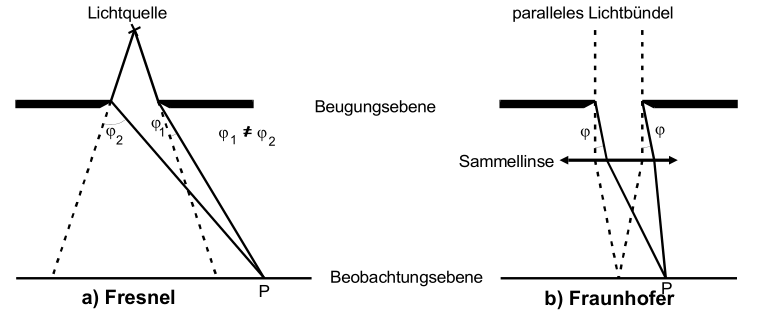
\includegraphics[width=0.5\textwidth]{latex/images/fresnel.PNG}
        \caption{Fresnelsche und Fraunhofersche Beugung an einem Spalt\protect \cite{V406}.}
        \label{img:fresnel}
    \end{figure}

    \noindent Bei der Fresnelschen Lichtbeugung am Spalt liegt die Lichtquelle in einer endlichen Entfernung vom Spalt und Beobachter, 
    damit nun zwei unterschiedliche Strahlenbündel an der gleichen Stelle auf dem Schirm ankommen, müssen sie am Spalt mit unterschiedlichen 
    Winkeln gebeugt werden. Bei der Frauenhoferschen Lichtbeugung liegt die Lichtquelle und der Beobachter im unendlichen, so dass die eingehende Welle durch 
    eine ebene Welle beschreiben werden kann. Weiterhin werden die Strahl hinter dem Spalt durch eine Sammellinse gebündelt, somit wird 
    erreicht, dass die unterschiedlichen Lichtbündel die im Punkt P interferieren, mit dem gleichem Winkel gebeugt werden. Der Parallelspalt 
    wird im folgenden mit der Frauenhofer Lichtbeugung betrachtet.

    \subsection{Parallelspalt}

        \noindent Hier wird ein Spalt mit hoher Länge im vergleich zur Breite genutzt, somit wird die Beugung auf eine Dimension beschränkt.
        Die Feldstärke der einfallenden ebenen Welle wird durch 

        \begin{equation*}
            A(z,t) = A_0 \text{exp}\left(i \omega t - \frac{i 2\pi z}{\lambda}\right)
        \end{equation*}

        \noindent mit der Zeit $t$ und dem Abstand in Z-Richtung $z$ beschrieben. Licht dieser Art kann mit einem Laser erstellt werden, 
        dieser liegt nicht in der unendlich großer Entfernung, sondern in einer Entfernung die groß im Vergleich zur Spaltbreite ist. 
        Das erscheinende Beugungsbild lässt sich mittels dem Huygenschen Prinzip der Elementarwellen und dem Interferenzprinzip 
        erklären. A. Fresnel schrieb erstmalig in 1818: Jeder Punkt einer Wellenfläche sendet zur gleichen Zeit sogenannte Elementarwellen aus, 
        die die Form von Kugelwellen haben. Diese Wellen interferieren miteinander und erzeugen eine neue Wellenfront, die gleich der Einhüllenden
        der Elementarwelle ist. Um nun den Schwingzustand in einem Punkt zu bestimmen, werden sämtliche Elementarwellen die in einem Punkt zusammen 
        laufen überlagert.

        \begin{figure}[ht]
            \centering
            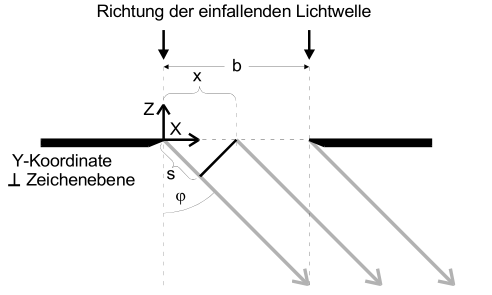
\includegraphics[width=0.5\textwidth]{latex/images/einzel.PNG}
            \caption{Fresnelsche und Fraunhofersche Beugung an einem Spalt\protect \cite{V406}.}
            \label{img:einzel}
        \end{figure}

        \noindent Wird nun die Amplitude einer in Richtung $\varphi$ gebeugten Welle betrachtet, müssen alle Strahlbündel die an jedem Punkt der 
        Spaltöffnung emittiert werden, summiert werden. Sie alle wurden in $\varphi$ Richtung gebeugt, haben aber einen Phasendifferenz 

        \begin{equation*}
            \delta = \frac{2 \pi s}{\lambda} = \frac{2 \pi x \text{ sin}(\varphi)}{\lambda}.
        \end{equation*}

        \noindent Da die einzelnen Strahlenbündel auf einer infinitesimal kleinen Breite d$x$ entstehen, kann die Amplitude $B$ in 
        $\varphi$ Richtung mittels des Integrals 
        
        \begin{align*}
            B(z,t,\varphi) &= A_0 \cdot \int_0^b \text{exp}\left\{ i \left( \omega t - \frac{2 \pi z}{\lambda} + \delta \right) \right\} \text{d}x \\
                           &= A_0 \cdot \text{exp}\left\{ i \left( \omega t - \frac{2 \pi z}{\lambda} \right) \right\} \cdot \int_0^b 
                           \text{exp}\left( \frac{2 \pi i x \text{ sin} (\varphi)}{\lambda }\right) \text{d}x
        \end{align*}

        \noindent berechnet werden. Wird das Integral ausgerechnet und die Eulersche Formel $\text{ sin}(\alpha) = \frac{1}{2i}\left( 
        \text{e}^{i \alpha} - \text{e}^{-i \alpha} \right)$ eingsetzt, ergibt sich für die Amplitudenfunktion

        \begin{equation}
            B(z,t,\varphi) = A_0 \text{exp}\left\{ i \left( \omega t - \frac{2 \pi z}{\lambda} \right) \right\} \cdot
            \text{exp}\left\{ \frac{\pi i b \text{ sin}(\varphi)}{\lambda} \right\} \cdot \frac{\lambda}{\pi\text{ sin}(\varphi)}
            \text{ sin}\left\{ \frac{\pi b \text{ sin}(\varphi)}{\lambda} \right\}.
            \label{eqn:beug}
        \end{equation}

        \noindent Die erste Exponentialfunktion stellt nun die Zeit- und Ortsabhängigkeit dar, die zweite ist ein richtungsabängiger 
        Phasenfaktor. Von besonderer experimenteller Beduetung ist hier der letzte Faktor. Mittels der Substitution 

        \begin{equation*}
            \eta := \frac{\pi b \text{ sin}(\varphi)}{\lambda}
        \end{equation*}
        
        \noindent kann dieser als 

        \begin{equation*}
            B(\varphi) = A_0 b \frac{\text{ sin}(\eta)}{\eta}
        \end{equation*}

        \noindent dargestellt werden. Dies ist eine gerade Funktion mit unendlich vielen Nullstellen bei 

        \begin{equation*}
            \text{ sin}(\varphi_n) = \pm n \frac{\lambda}{b}
        \end{equation*}

        \noindent und fallender Amplitude mit wachsendem $\eta$. Eine solche Funktion ist in Abbildung(\ref{img:Amplitude}) dargestellt.

        \begin{figure}[ht]
            \centering
            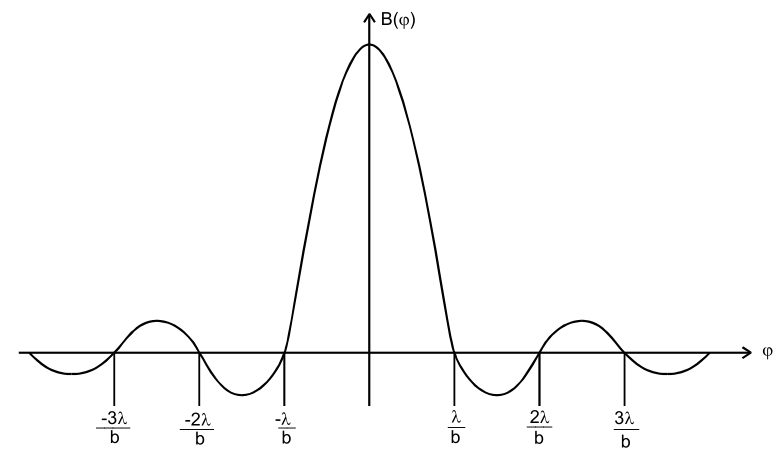
\includegraphics[width=0.5\textwidth]{latex/images/Amplitude.PNG}
            \caption{Amplitude einer an einem Parallelspalt gebeugten, ebenen Welle\protect \cite{V406}.}
            \label{img:Amplitude}
        \end{figure}

        \noindent Aufgrund der hohen Lichtfrequenz des Lichts ist es jedoch nicht möglich die Amplitude einer einzelnen Welle zu messen. 
        In diesem Versuch wird somit die zeitlich gemittelte Intensität betrachtet, diese wird durch 

        \begin{equation}
            I(\varphi) \propto B(\varphi)^2 = A_0^2 \left\{ \frac{\lambda}{\pi b \text{ sin}(\varphi)} \right\}^2 \cdot \text{ sin}^2 
            \left\{\frac{\pi b \text{ sin}(\varphi)}{\lambda} \right\}
            \label{eqn:einzel}
        \end{equation}

        \noindent beschrieben. Diese ist minimiert bei den Nullstellen der Amplitudenfunktion(\ref{eqn:beug}), die Maxima nehmen wiederum 
        mit dem Quadrat des Beugungswinkel ab.

    \subsection{Doppelspalt}

        \noindent Wird das Integral über die Spalt Öffnung analog zum Einzelspalt integriert, entsteht beim 
        Doppelspalt(siehe Abbildung(\ref{img:Doppelspalt})) die Intensitätsverteilung

        \begin{figure}[ht]
            \centering
            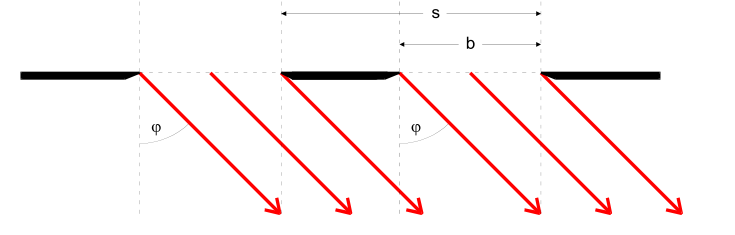
\includegraphics[width=0.5\textwidth]{latex/images/Doppelspalt.PNG}
            \caption{Beugung am Doppelspalt.\protect \cite{V406}.}
            \label{img:Doppelspalt}
        \end{figure}

        \begin{equation}
            I(\varphi) \propto B(\varphi)^2 = 4 \cdot \text{cos}^2 \left( \frac{\pi s \text{ sin}(\varphi)}{\lambda} \right) \cdot 
            \left\{ \frac{\lambda}{\pi b \text{ sin}(\varphi)} \right\}^2 \cdot \text{ sin}^2 \left\{ \frac{ \pi b \text{ sin}}{\lambda} \right\}^2 .
        \end{equation}

        \noindent Diese setzt sich aus der Intensitätsverteilung des Einzelspaltes(\ref{eqn:einzel}) und einer $\text{cos}^2$-Verteilung zusammen. Die 
        Minima dieser Verteilung  sind nun die gleichen des Einzelspaltes und die Nullstellen der $\text{cos}^2$-Verteilung bei 

        \begin{equation*}
            \varphi(k) = \text{arc sin}\left( \frac{2k +1 }{2s} \right) \cdot \lambda .
        \end{equation*}

    \subsection{Fraunhofersche Beugung und Fourier-Transformation}

        \noindent Die Amplitudenverteilung bei der Frauenhofer Beugung lässt sich auch allgemeiner mittels einer Fourier-Transformation 
        berechnen, dazu wird die einfallende Welle in der Beugungsebene, die Aperturfunktion transformiert.
        Allgemein wird die Fouriertransformation durch den Ausdruck 

        \begin{equation}
            \label{eqn:Fourier}
            g(\xi) := \int_{-\infty}^{+\infty} f(x) \text{e}^{i x \xi} \text{d}x
        \end{equation}

        \noindent beschrieben, angewandt auf die Aperturfunktion des Spalts der breite b 

        \begin{align*}
            f(x) & = A_0 \quad & \text{für } 0\leq x \leq b\\
            f(x) & = 0 \quad & \text{sonst}
        \end{align*}

        \noindent ergibt die Fouriertransformation

        \begin{equation*}
            g(\xi) := \int_{-\infty}^{+\infty} f(x) \text{e}^{i x \xi} \text{d} x = A_0 \cdot \int_0^b \text{e}^{i x \xi} \text{d} x =
            \frac{A_0}{i \xi} \left( -1 + \text{e}^{i \xi b} \right) .
        \end{equation*}

        \noindent Mittels der Eulerschen Formel ergibt sich hieraus 

        \begin{equation*}
            g(\xi) = \frac{2 A_0}{\xi} \text{exp} \left( \frac{i \xi b}{2} \right) \text{ sin} \left( \frac{\xi b}{2} \right) .
        \end{equation*}

        \noindent Wird hier die Substitution 

        \begin{equation}
            \xi := \frac{2 \pi \text{ sin}(\varphi)}{2} 
        \end{equation}

        \noindent durchgeführt, ergibt sich die bereits berechnete Amplitudenfunktion für den Einzelspalt(\ref{eqn:beug}).
        Es izt zu erkennen, dass die Fourier-Transformation das Huygensche Prinzip mathematisch formuliert, denn der Faktor 
        $\text{e}^{i x \xi}$ beschreibt die Phasendiffernz die durch $x$ entsteht. Mittels einer zwei oder mehrdimensionalen 
        Aperturfunktion kann also über die Fouriertransformation die Beugung an einem zweidimensionalen Objekt berechnet werden. 
        Umgekehrt lässt sich somit auch über die Amplitudenfunktion die Aperturfunktion, also die Form des Objekts berechnen.


        



    





    